%!TEX root = thesis.tex

\documentclass[a4paper]{article}
\usepackage{amsthm}
\usepackage[utf8]{inputenc}
\usepackage{csquotes}
\usepackage[english]{babel}
\usepackage{graphicx}
\usepackage{enumitem}
\usepackage{subcaption}  %ALLOWS SUBFIGURES
\usepackage{wrapfig}

\usepackage[draft]{fixme}
\fxsetup{theme = color}
\definecolor{fxnote}{rgb}{0.0000, 0.6000,0.0000}
\definecolor{fxwarning}{rgb}{1.0000,0.5490,0.0000}
\definecolor{fxerror}{rgb}{1.0000,0.2706,0.0000}
\definecolor{fxfatal}{rgb}{1.0000,0.0000,0.0000}
\usepackage[backend=biber, giveninits =true, isbn=false, url=false, maxbibnames=100]{biblatex}
\usepackage{hyperref}

%Theorems
\newtheorem{thrm}{Theorem}
\newtheorem{lemma}[thrm]{Lemma}
\newtheorem{prop}[thrm]{Proposition}
\newtheorem{remark}[thrm]{Remark}

\theoremstyle{definition}
\newtheorem*{defi}{Definition}

%%BeginIpePreamble
\usepackage{amsmath}
\usepackage{amssymb}
\usepackage{amsopn}

\newcommand{\scr}[1]{\mathcal{#1}}
\newcommand{\Z}{\mathbb{Z}}
\newcommand{\F}{\mathbb{F}}
\newcommand{\R}{\mathbb{R}}
\newcommand{\N}{\mathbb{N}}
\newcommand{\Q}{\mathbb{Q}}


%Operators
\newcommand{\id}{\operatorname{Id}}



%braces etc
\newcommand{\braces}[1]{\left\lbrace {#1} \right\rbrace}
\newcommand{\sqbr}[1]{\left\lbrack {#1} \right\rbrack }
\newcommand{\abs}[1]{\left\lvert {#1} \right\rvert }
\newcommand{\ceil}[1]{\left\lceil{ #1 } \right\rceil}
\newcommand{\floor}[1]{\left \lfloor {#1}\right\rfloor}
\newcommand{\parens}[1]{\left( {#1} \right)}


%utility
\newcommand{\inv}[1]{{#1}^{-1}}
\newcommand{\half}{\frac{1}{2}}
\newcommand{\third}{\frac{1}{3}}
\newcommand{\goes}{\rightarrow}
\newcommand{\nin}{\not \in}
\newcommand{\sm}[1]{\setminus \braces{#1} }

%vectors and matrices
\newcommand{\zerov}{\vec{0}}
\newcommand{\onev}{\vec{1}}

\newcommand{\twovec}[2]{\parens{ \begin{array}{c}#1 \\ #2\end{array} }}
\newcommand{\threevec}[3]{\prens{ \begin{array}{c}#1 \\ #2\\#3 \end{array} }}
\newcommand{\fourvec}[4]{\parens{ \begin{arr\newcommand{\ifftext}{if and only if }ay}{c}#1 \\ #2\\#3\\#4 \end{array} }}
\newcommand{\twomatrix}[4]{\parens{\begin{array}{cc}#1 & #2 \\ #3 & #4 \end{array}  }}
\newcommand{\twodiagmatrix}[2]{\parens{\begin{array}{cc}#1 & 0 \\ 0 & #2 \end{array}  }}

%%%%THIS THESIS
\newcommand{\intplus}{\operatorname{Int^{+}}}
\newcommand{\interior}{\operatorname{Int}}
\newcommand{\spl}{\operatorname{split}}
\newcommand{\mrg}{\operatorname{merge}}


\newcommand{\ext}[1]{\bar{#1}}
\newcommand{\tightext}[1]{\bar{#1}_t}
\newcommand{\dualgraph}[1]{\G(#1)}
\newcommand{\extdualgraph}[1]{\G_{\scr E}(#1)}



\newcommand{\W}{\scr W}
\renewcommand{\P}{\scr P}
\newcommand{\C}{\scr C}
\newcommand\restrict[1]{\raisebox{-.5ex}{$|$}_{#1}}
\newcommand{\restC}[1]{\ensuremath{\C\restrict{#1}}}

%p is for pole
\newcommand{\pN}{\mathrm{N}}
\newcommand{\pS}{\mathrm{S}}
\newcommand{\pE}{\mathrm{E}}
\newcommand{\pW}{\mathrm{W}}

\newcommand{\cpath}{\C \setminus \braces{\pS}} %cycle path

\newcommand{\rel}{\text{regular edge labeling }}

%%EndIpePreamble


%bib stuff
\bibstyle{plain}


%invariant enviroment
\newenvironment{invariants}{%
  \refstepcounter{thrm}%
  \paragraph{Invariants~\theprop}%
  \renewcommand*{\theenumi}{\theprop\,(I\arabic{enumi})}%
  \renewcommand*{\labelenumi}{(I\arabic{enumi})}%
  \enumerate
}{%
  \endenumerate
}

\begin{document}

\section{Algorithms}
Kant and He \cite{KH} were the first to desing algorithms that determine a regular edge labeling. 

Fusy \cite{Fusy2006, Fusy2009} recently developed a different algorithm computing a specific regular edge labeling using a method shrinkg a sweepcycle while coloring the outside in accordance with a regular edge labeling.\footnote{The specific regular edge labelling Fusy obtained was the minimal element of the lattice of regular edge labellings.}

All algorithms in this section will have the same core (based on \cite{Fusy2006}). Consisitng of shrinking a sweepcycle by socalled \emph{valid} paths\footnote{In Fusy's work these are called \emph{eligible paths}}. But will differ in which valid paths they choose (if there are multiple).


We will start this section with some notation and preliminaries in Subsection \ref{ss:not}. Then we will state the core algorithm and show that it always computes a regular edge labeling in Subsection \ref{ss:core}. Afterwards we show in Subsections \ref{ss:minimal}, \ref{ss:blue}, \ref{ss:red}. How one can adapt the choice of the valid paths to obtain regular edge labellings with certain properties. \fxnote{what properties}


\subsection{Notation and Preliminaries}
\label{ss:not}
\begin{defi}[Interior path]
We call a path $P$ an internal path of a cycle $C$ if all its edges are in the interior\fxnote{is interior defined somewhere?} of $C$ and it connects two distinct vertices of $C$ 
\end{defi}

We will use a script $\C$ to indicate the current sweep cycle. 
We will repeatedly only consider the path $\cpath$. In that case we will always order it from $\pW$ to $\pE$. 

We will let $\P$ denote a interior path. Given such a path of $k$ vertices we will index it's nodes by $p_1, \ldots, p_k$ in such a way that $p_1$ is closer to $\pW$ then $p_k$ is (and thus that $p_k$ is closer to $\pE$ then $p_1$ is). 

Then $p_1$ and $p_k$ indicate the two unique vertices of the walk that are also part of the cycle. We will then let $\restC{\P}$ denote the part of $\cpath$ that is between $p_1$ and $p_k$ (including). $\C_\P$ will denote the cycle we get when we paste $\restC{\P}$ and $\P$.



\subsection{Core}
\label{ss:core}

The algorithm will always maintain the following three invariants

\begin{invariants}
  \itemsep=-4pt

\item \label{i:1} The cycle $\C$ contains the two edges $\pS \pW$ and $\pS \pE$.
\item \label{i:2} $\cpath$ has no chords in it's interior \fxwarning{def chord and chord in interior (or just simplify to has no chords}
\item \label{i:last} All inner edges of $T$ outside of $\C$ are colored and oriented in such that the innnervertex condition holds. %TODO what is the inner vertex condition
\end{invariants}

A cycle satisfying these three invariants will have the same general shape as in figure \ref{fig:invCycle}. We note that the cycle has at least $4$ vertices because otherwise a seperating triangle is created. 

\begin{figure}[h!]
\centering
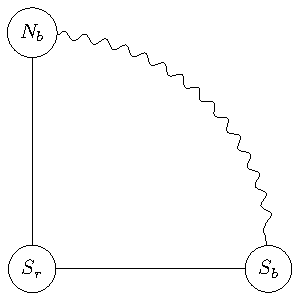
\includegraphics{img/invCycle}

\caption{An example of a cycle $\C$ satisfying the invariants 
    \label{fig:invCycle}}
\end{figure}

It is also nice to note that the union of the cycle and it's interior form a triangulation of the $n$-gon since it is a induced subgraph of a triangulation of the $4$-gon.


\subsubsection{Eligible paths}



\begin{defi}[valid path]
We call an internal path $\P$ from $w_1$ to $w_k$ valid if 
\begin{enumerate}
 \renewcommand*{\labelenumi}{(E\arabic{enumi})}%
 \renewcommand*{\theenumi}{(E\arabic{enumi})}%


\item Neither $w_1$ or $w_k$ is $\pS$ \label{e:notSr}
\item The paths $\P$ and $\restC \P$ both are more then 1 edge \footnote{i.e. both have an interior vertex} \label{e:length2borders}
\item Each edge in the interior to $\C_\P$ connects a vertex of $\P\setminus{\braces{w_1,w_k}}$ and $\restC \W \setminus{\braces{w_1,w_k}}$. In particular $\C_\P$ is a non-separating cycle.
\label{e:crossingedge}
\item The cycle $\C'$ obtained by replacing $\restC \P$ by $\P$ in $\C$ has no chord that doesn't involve $\pS$.
\label{e:noChordinC'}
\end{enumerate}
\end{defi}

\begin{remark}
``Shrinking'' the cycle with an eligible path will keep all the invariants true.
\end{remark}

We will show the following proposition.


\fxfatal{This is very hard to prove, mustly the part that we can always find a path satisfying E4. See page 11. Prrof this from red algo.}
\begin{thrm}[Existence of a eligible path]
\label{th:eligExistence}
When the algorithm's invariant (\ref{i:1} - \ref{i:last}) are satisfied and the cycle $\C$ is separating then there exist a \emph{eligible} internal path.
\end{thrm}

\begin{proof}
We will first show that there always exists an internal path $\P$. We will then show that a internal path can be found that satisfies conditions $(E1) - (E4)$.

In the proof we will often use that a 

Let us first note that if the cycle $C$ is separating (i.e has a non-empty interior), there is at least one interior vertex $v$. Since the triangulation of a $n$-gon is $2$-connected there are two ways to go from $v$ to (say) $S_r$. Hence there is an internal path $\P_0$.
%TODO this is not true, luckily we can use the connections to cyle lemma

If this path does not satisfy \ref{e:notSr} we can use the following construction. The other vertex where $P_0$ intersects $\C$ is not $S_r$. Let us call this vertex $x$ and it's neighbour on the path $y$. The vertex $x$ might be $N_b$ or $S_b$ but can't be both, hence it has at least one neighbour $z$ on the cycle that is not $S_r$. Because the triangulation of a $n$-gon is internally maximally planar we have that $yz$ is an edge. Now $xyz$ is an internal path satisfying \ref{e:notSr}. See also figure \ref{fig:E1}, here we made a choice on which side of $y$ the vertex $z$ lies, but this choice can be made without losing generality.

Hence we have now constructed, or already had, a path that satisfies \ref{e:notSr}. Let us for the remainder of the proof denote this path by $\P_1$.


\begin{figure}[ht]
\centering
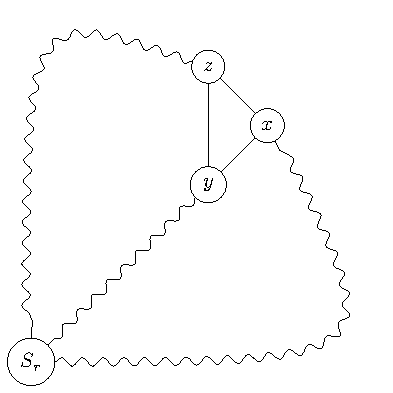
\includegraphics[]{img/E1}
\caption{Constructing a path satisfying \ref{e:notSr} \label{fig:E1}}
\end{figure}

\paragraph{There is a path that also satsifies (E2)}
If $\P_1$ satisfies (E2) we set $\P_2 = \P_1$ otherwise we will create a path that satisfies (E1) and (E2). 
If the path $\P_1$ does not satisfy $(E2)$ \footnote{which will be the case if the above construction has been used} then there are two possibilities  a) $\P_1$ does not have interior vertices and/or b) $[v,v']$ does not have interior vertices. If a) would be true the existence of $P_0$ would contradict Invariant \ref{i:2}. Hence the only problem can be that $b)$ occurs. 

If $v=N_b$ and $v'=S_b$ we have found a separating triangle given by $S_rN_bS_b$ \footnote{this is the cycle $\C$ which is separating} in original graph. Hence at least one of $v$ or $v'$ is not $N_b$ or $S_b$. If we call this vertex $x$ its neighbour on the path $y$ and it's neighbour outside $[v,v']$ $z$. We see that by the interior of $\C$ being maximally planar $yz$ must be an edge. If we now adapt $P_1$ by replacing $yx$ by $yz$ we have made $[v,v']$ one vertex longer and hence created a path satisfying \ref{e:length2borders}. In figure \ref{fig:E2} we show this procedure in two cases. Executing this procedure does not change that $S_r$ is not one of the endpoints of the path. Hence we have now created a path $\P_2$ that satisfies \ref{e:notSr} and \ref{e:length2borders}.

\begin{figure}
    \centering
    \begin{subfigure}[b]{0.45\textwidth}
        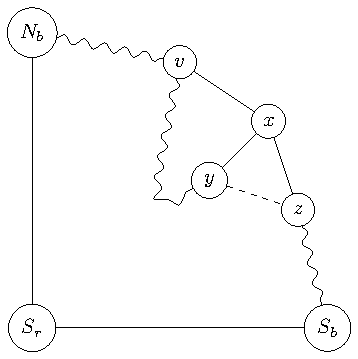
\includegraphics[width=\textwidth]{img/E2general}
        \caption{The general case. Note that $x=v'$.}
    \end{subfigure}
    ~ 
    \begin{subfigure}[b]{0.45\textwidth}
        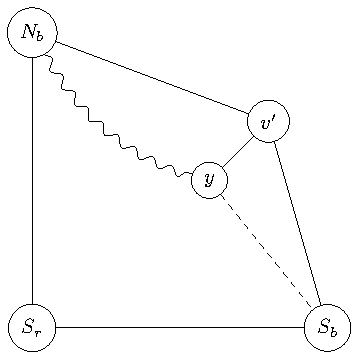
\includegraphics[width=\textwidth]{img/E2spec}
        \caption{A specific case. Note now that $N_b=v, v'=x$ and $S_b=z$}
    \end{subfigure}

    \caption{Creating a path satisfying \ref{e:length2borders}. The dotted line is the edge we take in the new path $\P_2$}\label{fig:E2}
\end{figure}

\newcommand{\intvv}{\ensuremath{[v,v']\setminus{v,v'}}}
\newcommand{\intP}{\ensuremath{\P\setminus{v,v'}}}

\paragraph{There is a path that also satisfies (E3)}
If $\P_2$ satisfies $(E3)$, we take $\P_3 = \P_2$. Otherwise we will remedy the defect. We separate five different cases of offending edges. All of the five cases will be easy to remedy giving a path $\P'_2$ still satisfying \ref{e:notSr} and \ref{e:length2borders} such that $\C_{\P'_2}$ is strictly contained in $\C_{\P_2}$ %Q what is the right version of smaller here?
\begin{enumerate}
 \renewcommand*{\labelenumi}{\alph{enumi})}%
 \renewcommand*{\theenumi}{\alph{enumi})}%
 \item edges from \intvv to $\intvv$
 \item edges from $\intP$ to $\intP$
 \item edges incident to $v$ or $v$ and some other vertex on $\C_{\P_2}$
 \item edges from $[v,v']$ to some internal vertex 
 \item edges from $\intP$ to some internal vertex
\end{enumerate}

The existence of an edge as in a) is forbidden by Invariant \ref{i:2}. If b) occurs we can simply shortcut our original path $\P_2$ with this edge. If c) occurs this edge can't go to another vertex in $[v,v']$ since that would offend Invariant \ref{i:2}. Hence they go to a vertex in $\P_2$ and we can shortcut the path as in b).

If d) occurs we simply make a new path and if e) occurs we take a slightly adapted interior path. See figures

%TODO pictures

Since all of the moves shrink $\C_{\P_2}$ while keeping \ref{e:notSr} and \ref{e:length2borders} intact and we can't infinitely shrink this means at a certain point no more moves are available. Since every offending edges allows a move this means that there are no more offending edges. Hence this version of $\P'_2$ satisfies \ref{e:crossingedge}. For the final step of the proof we take $\P_3 = \P'_2$.

%TODO formulate repetition argument nicly

\paragraph{There is a path that also satisfies \ref{e:noChordinC'}}
Suppose that $\P_3$ does not satisfy \ref{e:noChordinC'}. Then we can just take the would be interior edge and take this for a nwe path. This is again a finite procedure reducing the sum of $|\P_3| -|[v,v']|$. In the end we have a path satisfying \ref{e:notSr} - \ref{e:noChordinC'}.

%TODO picturse, why dont we lose E1-E3


\end{proof}

\subsection{Minimum distributive lattice element}
\label{ss:minimal}
We get this when we take the    ``leftmost'' eligible path. 
\fxnote{write section, potentially just refer to Fusy2006}

\renewcommand{\F}{\scr F}
\subsection{Horizontal one-sides}
\label{ss:blue}
\note we should define the border of a face of a bipolar orientation somewhere. 
\note and what we mean with \emph{cycle border} and \emph{face border}
\note as well as the notation of $\F_\P$ the face of a path

As an exercise one could try to addapt Fusy's algorithm to generate horizontally one-sided layouts directly, without doing flips in the distributive lattice. It turns out that this is not that diffcult.

Since the horizontal segments correspond to face in the blue bipolar orientation we want that one of the two borders of the face has a length of at most two. Since every eligible path we take splits off one face in the blue bipoolar orientation it is easy to control this property.

\begin{thrm}
\label{th:blueelig}
In the update of the algorithm there is always an eligible path $\P$ available such that either $\P$ or $[v,v']$ is of length $2$. 
\end{thrm}

In order to proof this theorhem we will first show the following lemma.

\begin{lemma}
\label{lem:bluealgo}
If $\P$ is an eligble path giving raise to a face $\F_P$ of which both border have length at least $3$. Then there exist an eligible path $\P'$ such that the pathborder and cycleborder of its face $\F_{\P'}$ are both at least $1$ shorter than those of $\F_\P$.
\end{lemma}

\begin{proof}
In this proof we will frequently use property \ref{e:crossingedge} of a Eligible path, we won't mention it every time we use it.

We denote the source by $s$ and the sink by $t$. We also assign names$a, b$ and $x, y$ to the first two vertices on both borders, see Figure \ref{bluefig:notation}. Since every interior face of $G$ is a triangle $ax$ is an edge. Now we distinguis two cases, either $ay$ is an edge (case 1) or $bx$ is an edge (case 2). Tey can't both be an edge at the same time due to planarity, neither can it happen that both of them are not an edge since then the face containing the path $baxy$ is at least of degree $4$.

In the first case $a$ may be connected to more vertices on the pathborder, however there is a last one, say $z$. And this vertex is then also connected to $b$, otherwise it would not be the last one. Now we can provide an shorther eligible path $\P'$ we start at $a$ go to $z$ and from there we follow the old path $\P$ to $t$.  See figure \ref{bluefig:case1}. It is easy to see that all four properties of an eligible path hold for $\P'$.
\begin{comment}
By construction $\P'$ satifies \ref{e:notSr} and \ref{e:internalVertices}. While the interior of $\C_{\P'}$ is a subset of that $\C_\P$%TODO this is again an eligible path
\end{comment}

In the second case $x$ may be connected to more vertices along the cycle border, however there is a last one, say $c$. And this vertex is then also connected to $y$, otherwise it would not be the last one. Now we can provide an shorther eligible path $\P' = sxz$.   See figure \ref{bluefig:case2}. It is straightforward to see that all four properties of an eligible path hold for $\P'$. %TODO this is again an eligible path
\end{proof}

\begin{figure}[ht]
    \centering
    \begin{subfigure}[b]{0.45\textwidth}
        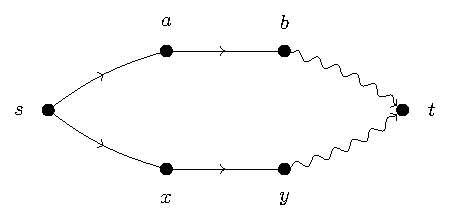
\includegraphics[width=\textwidth]{img/blue/setting}
        \caption{The setting}
        \label{bluefig:notation}
    \end{subfigure}
    
    \begin{subfigure}[b]{0.45\textwidth}
        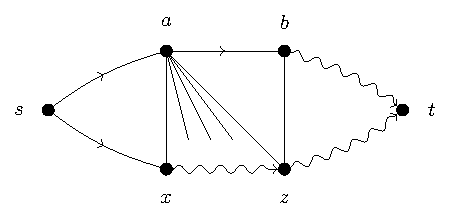
\includegraphics[width=\textwidth]{img/blue/case1}
        \caption{Case 1}
        \label{bluefig:case1}
    \end{subfigure}
    ~
    \begin{subfigure}[b]{0.45\textwidth}
        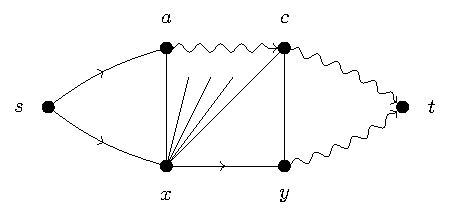
\includegraphics[width=\textwidth]{img/blue/case2}
        \caption{Case 2}
        \label{bluefig:case2}
    \end{subfigure}

    	\caption{}
\end{figure}

\begin{proof}[Proof of Theorem \ref{th:blueelig}]
By Theorem \ref{th:eligExistence} we know there is a eligible path $\P$. If one of the borders of $\F_\P$ is of length $2$ or less we are done. If this path gives raise to a face $\F_\P$ with both borders are both of length at least $3$ we can repeatedly apply Lemma \ref{lem:bluealgo} until at least one of the borders is of length at most $2$. 
\end{proof}

If we in every update of the algorithm take the paths from Theorem  \ref{th:blueelig} we end up with the correct faces in the blue bipolar orientation and hence a horizontally one sided rectangular dual.

\subsection{Vertical one-sided}
\label{ss:red}

We can also adapt Fusy's algorithm to generate a vertically one-sided dual. We do this by picking the eligible path with the leftmost starting point and letting it run for as long as possible. In the final oriented regular edge labelling we want to prevent red faces that have $3$ or more edges on both borders. 

If a red face has 
\begin{lemma}
A face $F$ with at least $3$ edges on each side contains a $Z$ 
\end{lemma}

But a $z$ can only be the result of a seqeuncce of eligble paths that does not satisfy the requirements. 

\end{document}